\documentclass{article}
\usepackage{graphicx}
\usepackage{wrapfig}
\usepackage[utf8]{inputenc}
\usepackage[english]{babel}

\graphicspath{ {pic/} }
\begin{document}

%\title{OSVVM - FIFO (scoreboard)}
%\maketitle
%\begin{\figure}[h]
%
\includegraphics[width=3cm, height=4cm]{jl}
%\end{figure}

%\centering {\huge\bfseries OSVVM - FIFO (scoreboard)\par}
\section{OSVVM - FIFO (scoreboard)}
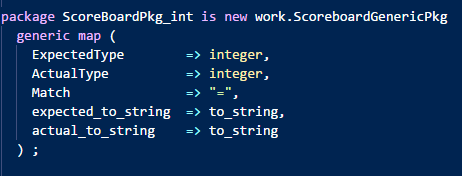
\includegraphics[scale=0.8]{sb_int}\\
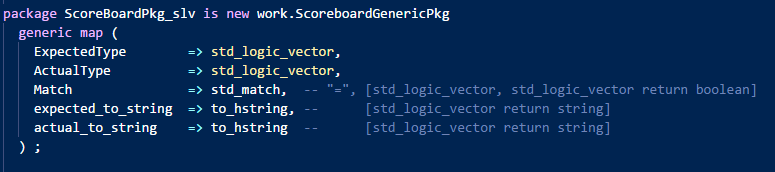
\includegraphics[scale=0.8]{sb_slv}\\
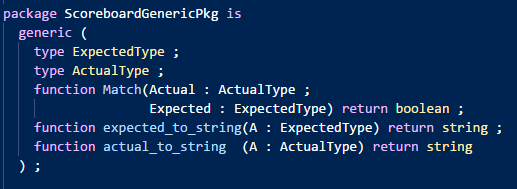
\includegraphics[scale=0.8]{sb_generic}\\
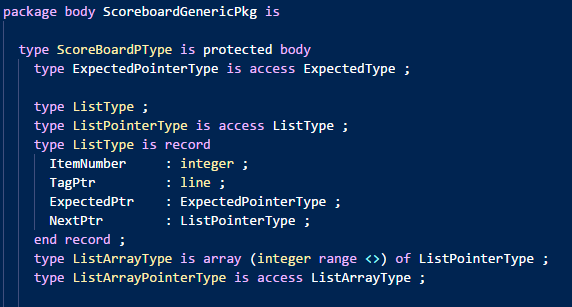
\includegraphics[scale=0.8]{sb_body}\\

\newpage
\noindent
``The scoreboard package uses package generics to allow the test value type and receive value type to 
be changed. Furthermore the function to compare the test value with the receive value is pass as a 
subprogram generic to allow more complicated checking than a simple ``='' to be done. In addition 

\begin{wrapfigure}{r}{0.25\textwidth}
  \centering
  
\includegraphics[width=0.25\textwidth]{jl}
\end{wrapfigure}
\noindent
there are functions expected\_to\_string and actual\_to\_string to help printing the values of Expected type 
and ActualType respectively.''\\
\noindent
``Tagged Scoreboards are usd for systems that allow transactions to execute out of order. Tags are represented 
as string values (since most types convert to string using to\_string.''\\

\noindent
\textbf{shared variable SB : ScoreBoardPType;} or\\
\textbf{shared variable SB\_uart : work.ScoreBoardPkg\_Uart.ScoreboardPType;}\\

\noindent
SB.Push(ExpectedVal); SB.Check(ReceiveVal); SB.Pop(ExpectedVal);\\

\noindent
\textbf{\underline{ScoreboardGenericPkg}}\\
-- simple version\\
procedure push( item : in ExpectedType);\\
procedure push( constant tag : in string;\\
                constant item : in ExpectedType);\\
-- array version


\end{document}
